
\subsection{Cơ sở lý thuyết xây dựng phần cứng}

% Slide 1: Tổng quan hệ thống
\begin{frame}{Tổng quan Kiến trúc Hệ thống Phát hiện Té ngã}
\begin{block}{Phân loại hệ thống}
\begin{itemize}
\item \textbf{Dựa trên Camera}: Xử lý hình ảnh cố định, yêu cầu máy chủ mạnh
\item \textbf{Dựa trên Thiết bị đeo}: Cảm biến IMU, ESP32, truyền thông di động
\end{itemize}
\end{block}

\begin{block}{Ba thành phần cốt lõi}
\begin{enumerate}
\item \textbf{Thiết bị Thu thập Dữ liệu}: IMU, Camera, GPS
\item \textbf{Máy chủ/Xử lý}: Phân tích dữ liệu, Học sâu
\item \textbf{Truyền thông}: Wi-Fi, 4G/LTE đảm bảo kết nối
\end{enumerate}
\end{block}
\end{frame}

% Slide 2: ESP32
\begin{frame}{Vi điều khiển ESP32}
\begin{columns}
\column{0.6\textwidth}
\begin{block}{Đặc điểm chính}
\begin{itemize}
\item Lõi kép Xtensa LX6, FreeRTOS
\item Wi-Fi + Bluetooth tích hợp
\item Hỗ trợ MQTT, HTTP
\end{itemize}
\end{block}

\begin{block}{Phân công nhiệm vụ}
\begin{itemize}
\item \textbf{Lõi 1}: Xử lý thời gian thực (IMU, Kalman Filter)
\item \textbf{Lõi 2}: Truyền thông không dây
\end{itemize}
\end{block}

\column{0.4\textwidth}
\begin{center}
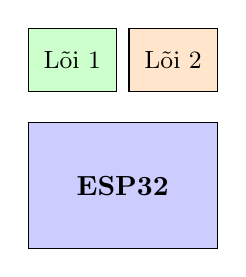
\begin{tikzpicture}[scale=0.8]
\draw[fill=blue!20] (0,0) rectangle (3,2);
\node at (1.5,1) {\textbf{ESP32}};
\draw[fill=green!20] (0,2.5) rectangle (1.4,3.5);
\node at (0.7,3) {\small Lõi 1};
\draw[fill=orange!20] (1.6,2.5) rectangle (3,3.5);
\node at (2.3,3) {\small Lõi 2};
\end{tikzpicture}
\end{center}
\end{columns}
\end{frame}

% Slide 3: IMU & GPS
\begin{frame}{Cảm biến IMU và GPS}
\begin{columns}
\column{0.5\textwidth}
\begin{block}{IMU}
\begin{itemize}
\item Gia tốc kế $\mathbf{a}=[a_x,a_y,a_z]$
\item Con quay hồi chuyển $\boldsymbol{\omega}=[\omega_x,\omega_y,\omega_z]$
\item Từ kế – xác định hướng
\item Fusion: Kalman/Madgwick
\end{itemize}
\end{block}

\column{0.5\textwidth}
\begin{exampleblock}{GPS}
\begin{itemize}
\item Module NEO-6M / EC800K
\item Định vị NMEA, tọa độ cứu hộ
\item Kết hợp truyền thông SMS/4G
\end{itemize}
\end{exampleblock}
\end{columns}
\end{frame}

% Slide 4: Thuật toán Phát hiện Té ngã
\begin{frame}{Thuật toán Phát hiện Té ngã}
\begin{columns}
\column{0.5\textwidth}
\begin{alertblock}{Shock Event}
$$\|\mathbf{a}\| > a_{\text{shock}}$$
Gia tốc tăng vọt đột ngột
\end{alertblock}

\column{0.5\textwidth}
\begin{alertblock}{Post-fall State}
\begin{itemize}
\item Gia tốc $\approx 1g$ (nằm yên)
\item Tốc độ góc thay đổi lớn
\end{itemize}
\end{alertblock}
\end{columns}
\end{frame}

% Slide 5: Edge vs Cloud
\begin{frame}{Xử lý tại Biên (Edge) và Máy chủ }
\begin{columns}
\column{0.5\textwidth}
\begin{block}{Edge (ESP32)}
\begin{itemize}
\item Xử lý IMU thời gian thực
\item Phát hiện té ngã sơ cấp
\item Truyền dữ liệu JSON/MQTT
\end{itemize}
\end{block}

\column{0.5\textwidth}
\begin{block}{Cloud/Server}
\begin{itemize}
\item Xử lý ảnh từ Camera (ESP32-S3 + OV5640)
\item TensorFlow/PyTorch, OpenCV
\end{itemize}
\end{block}
\end{columns}
\end{frame}

% Slide 6: Truyền thông
\begin{frame}{Hệ thống Truyền thông}
\begin{columns}
\column{0.5\textwidth}
\begin{alertblock}{Wi-Fi (chính)}
\begin{itemize}
\item Truyền tải dung lượng lớn (ảnh/video)
\item MQTT với máy chủ
\item Độ trễ thấp
\end{itemize}
\end{alertblock}

\column{0.5\textwidth}
\begin{alertblock}{4G/LTE (dự phòng)}
\begin{itemize}
\item SMS/cuộc gọi khẩn
\item Định vị GPS
\item Hoạt động khi Wi-Fi lỗi
\end{itemize}
\end{alertblock}
\end{columns}
\end{frame}

% Slide 7: Logic hoạt động
\begin{frame}{Logic Hoạt động Hệ thống}
\begin{enumerate}
\item ESP32 thu thập dữ liệu IMU/Camera
\item Phát hiện té ngã sơ cấp tại biên
\item Truyền dữ liệu lên máy chủ (ưu tiên Wi-Fi, dự phòng 4G)
\item Máy chủ xử lý tin và phát cảnh báo
\item Kích hoạt cảnh báo (SMS/cuộc gọi)
\end{enumerate}
\end{frame}

% Slide 8: Môi trường phát triển

\begin{frame}{Môi trường Phát triển (ESP-IDF)}
\begin{columns}
\column{0.5\textwidth}
\begin{block}{Đặc trưng của ESP-IDF}
\begin{itemize}
    \item \textbf{Build system CMake + Kconfig} 
          – cấu hình linh hoạt, dễ mở rộng component
    \item \textbf{FreeRTOS tích hợp sẵn} 
          – quản lý đa nhiệm trên 2 lõi Xtensa
    \item \textbf{Driver cấp thấp} 
          – I2C, SPI, UART, PWM, GPIO được tối ưu cho ESP32
    \item \textbf{Hỗ trợ mạng phong phú} 
          – Wi-Fi, Bluetooth, TCP/IP stack, MQTT, HTTP(S)
\end{itemize}
\end{block}

\column{0.5\textwidth}
\begin{exampleblock}{Lợi ích cho hệ thống Phát hiện Té ngã}
\begin{itemize}
    \item Quản lý \textbf{đa component} (IMU, SIM4G, LED, Fall Logic) độc lập
    \item Thực thi \textbf{song song}: 
          lõi 1 xử lý cảm biến, lõi 2 lo truyền thông
    \item Hỗ trợ \textbf{OTA update} để nâng cấp firmware từ xa
    \item Debug chuyên nghiệp: \texttt{idf.py monitor}, gdbstub, logging
\end{itemize}
\end{exampleblock}
\end{columns}
\end{frame}
